%!TEX root = ../Thesis.tex
\section{Test Setup} % (fold)
\label{sec:test_setup}


\subsection{Communication} % (fold)
\label{sub:communication}
The communication setup between the \gls{UAV}, landing pad, manual controller and the work station is illustrated in figure~\ref{fig:comSetupFig}.
\begin{figure}[ht]
    \centering
    \import{img/}{Communication.pdf_tex}
    \caption{Communication setup}
    \label{fig:comSetupFig}
\end{figure}
Figure~\ref{fig:comSetup} shows a photograph of the router, \gls{UAV}, and the \gls{CSU} used in the tests.
\begin{figure}[ht]
  \begin{center}
    \includegraphics[width=\linewidth]{img/communication.jpg}
        \caption{Router, UAV, CSU and landing pad}{Router, UAV, CSU and landing pad. Total setup for precise, autonomous landing}
        \label{fig:comSetup}
  \end{center}
\end{figure}

% subsection communication (end)

\subsection{Quadcopter} % (fold)
\label{sub:quadcopter}
The quadcopter used in this work is a 3DR Solo Drone produced by 3D Robotics photographed in figure~\ref{fig:UAV_closeup}. The UAV is a low cost commercial available quadcopter mainly used by hobbyists and photographers. In addition to the off the shelf quadcopter, a \gls{SBC}, a wireless adapter and a global shutter camera is connected to drone. Figure~\ref{fig:UAV_details} illustrates how the equipment is mounted on to the UAV and table~\ref{tab:partListquadcopter} lists the details of the equipment. The \gls{SBC} is running \gls{ROS} on Ubuntu 16.04 and communicates with the quadcopter using the mavROS interface \citep{mavros}.
\begin{figure}[!htb]
\centering
  \begin{minipage}{.54\textwidth}
    \centering
    \includegraphics[width=\linewidth]{img/UAV_closeup.jpeg}
    \caption{Closeup of the 3DR solo quadcopter}
    \label{fig:UAV_closeup}
  \end{minipage}%
  \hfill
  \begin{minipage}{.44\textwidth}
    \centering
    \includegraphics[width=\linewidth]{img/Uav_details.png}
    \caption{SBC, wireless adapter and camera mounted on the UAV}
    \label{fig:UAV_details}
  \end{minipage}
\end{figure}
\begin{table}[!htb]
  \centering
  \begin{tabular}{l l l}
    \toprule
    \textbf{Device}&\textbf{Brand}&\textbf{Type nr}\\ \hline
    Quadcopter&3D Robotics&SOLO Drone\\
    Single Board Computer&Hardkernel&ODROID-C2\\
    Wireless Adapter&Edimax&ew-7811uac\\
    Camera&iDS&UI-3250LE-C-HQ\\
    \bottomrule
  \end{tabular}
  \caption{List of Devices Quadcopter}
  \label{tab:partListquadcopter}
\end{table}


% subsection quadcopter (end)

\subsection{Landing Pads} % (fold)
\label{sub:landing_pad}
The fiducial marker used in this test setup, is a 80 times 80cm \gls{PRIAM} tag mounted on a wooden board. Tests have been carried out with the tag placed on the ground, at the back of the ground vehicle Olav and at the deck of the surface vehicle Odin. Both Olav and Odin have accurate navigation systems on board broadcasting the navigation data to the \gls{UAV}. In order to have a velocity and position measurement of the landing pad when using other landing pads, a \gls{CSU} where created in this work.
\begin{figure}[ht]
\centering
  \begin{minipage}{.46\textwidth}
    \centering
    \includegraphics[width=\linewidth]{img/landingOnOlavStatic.png}
    \caption{UAV landing on the FFI ground vehicle Olav}
    \label{fig:olavAndTag} 
  \end{minipage}%
  \hfill
  \begin{minipage}{.52\textwidth}
    \centering
    \includegraphics[width=\linewidth]{img/aruco_track_12m.png}
    \captionof{figure}{Olav detected from UAV camera at 12m}
    \label{fig:olavFrom12m}
  \end{minipage}
\end{figure}
\begin{figure}[ht]
\centering
  \begin{minipage}{.51\textwidth}
    \centering
    \includegraphics[width=\linewidth]{img/landingOnOdin.png}
    \caption{UAV landing on the FFI surface vehicle Odin}
    \label{fig:odinAndTag} 
  \end{minipage}%
  \hfill
  \begin{minipage}{.47\textwidth}
    \centering
    \includegraphics[width=\linewidth]{img/aruco_track_odin_15m.png}
    \captionof{figure}{Odin detected from UAV camera at 15m}
    \label{fig:odinFrom15m}
  \end{minipage}
\end{figure}

\subsubsection{Custom Sensor Unit} % (fold)
\label{ssub:custom_sensor_unit}
The \gls{CSU} is built by a flight controller, \gls{GNSS} sensor, \gls{SBC}, wireless adapter, battery and a 3D printed enclosure. Figure~\ref{fig:airTower} illustrates the included components in details. Detailed information of the components can be studied in table~\ref{tab:partListLandingPad}. The flight controller is running PX4 flight controller software communicating with the \gls{SBC} running Ubuntu 16.04 and \gls{ROS}. 
\begin{figure}[ht]
\centering
  \begin{minipage}{.49\textwidth}
    \centering
    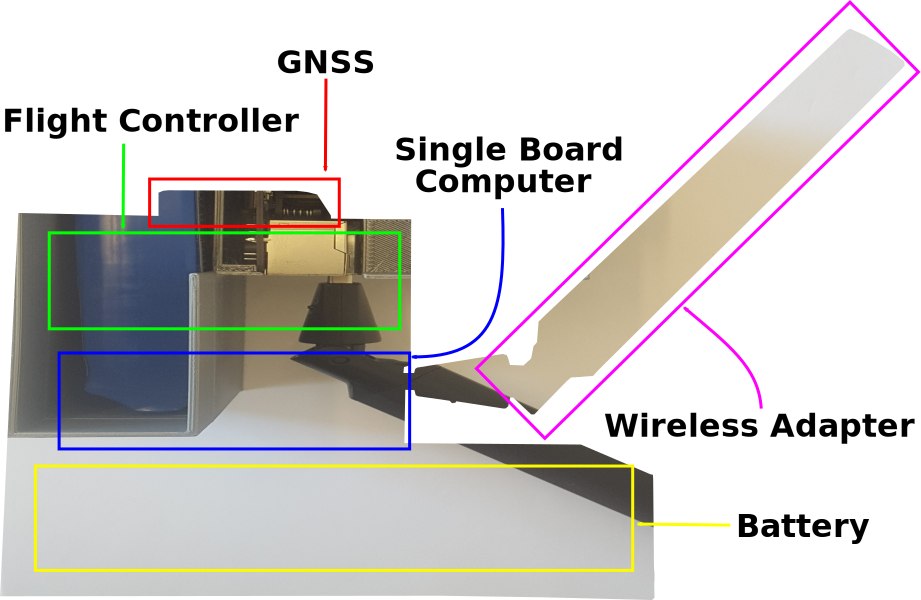
\includegraphics[width=\linewidth]{img/AirTower.png}
    \captionof{figure}{Overview of the components included in the SBC}
    \label{fig:airTower}
  \end{minipage}%
  \hfill
  \begin{minipage}{.49\textwidth}
    \centering
    \includegraphics[width=\linewidth]{img/airTraficControl.jpg}
    \captionof{figure}{Fully assembled SBC}
    \label{fig:airTowerBack}
  \end{minipage}
\end{figure}
\begin{table}[!htb]
  \centering
  \begin{tabular}{l l l}
    \toprule
    \textbf{Device}&\textbf{Brand}&\textbf{Type nr}\\ \hline
    GNSS sensor&mRo&GPS u-Blox Neo-M8N\\
    Flight Controller&mRo&Pixhawk 2.4.6\\
    Single Board Computer&Hardkernel&ODROID-C2\\
    Battery&Zippy Flightmax&3000mAh, 20C, 11.1v\\
    Wireless Adapter&Edimax&ew-7811uac\\
    \bottomrule
  \end{tabular}
  \caption{List of Devices in Custom Sensor Unit}
  \label{tab:partListLandingPad}
\end{table}
% subsubsection custom_sensor_unit (end)

% subsection landing_pad (end)
% section test_setup (end)



\section{Simulation Setup} % (fold)
\label{sec:simulation_setup}
A 2D simulation environment were developed to compare the two guidance methods developed in section~\ref{sec:guidance_methods}. The simulation environment were developed using Matlab and includes simplified dynamic models of Olav and the UAV. Moreover, Optimal and Parallel Navigation Guidance methods and a graphical illustration to present the results are implemented in the same environment.

The ground vehicle is modeled as the nonholonomic kinematic car based on rolling without slippering constraints given in \cite{spong2006robot} as
\begin{equation}
  \vect{\dot{q}}
  =
  \begin{bmatrix}
    0\\
    0\\
    0\\
    1
  \end{bmatrix}
  \phi
  +
  \begin{bmatrix}
    \cos(\theta)\\
    \sin(\theta)\\
    \frac{1}{d}\tan{\phi}\\
    0
  \end{bmatrix}
  \vect{v}^{n}_{l/n}
\end{equation}
with the state vector $\vect{q}$
\begin{equation}
  \vect{q}=
  \begin{bmatrix}
    p^n_{l/n,x}\\
    p^n_{l/n,y}\\
    \theta\\
    \phi
  \end{bmatrix}
\end{equation}
$\theta$ is the vehicle heading relative to the $n$ frame, $\phi$ is the vehicle steering angle, $\vect{p}^n_{l/n}\in\mathbb{R}^{2}$is the position of the landing pad relative to the $n$ frame, $\vect{v}^n_{l/n}\in\mathbb{R}^{2}$ is the landing pad velocity relative ti $n$ and $d$ is the length between the back and front wheels of the ground vehicle.

The UAV is modeled using a simple mass force model combined with a proportional velocity controller. The mass force model ca be given as
\begin{align}
  \vect{\dot{q}}&=
  \begin{bmatrix}
    \vect{v}^n_{u/n}\\
    \frac{\vect{f}_u^n}{m}
  \end{bmatrix}
  &
  \vect{q}&=
  \begin{bmatrix}
    \vect{p}^n_{u/n}\\
    \vect{v}^n_{u/n}
  \end{bmatrix}
\end{align}
where $\vect{p}^n_{u/n}\in\mathbb{R}^{2}$ and $\vect{v}^n_{u/n}\in\mathbb{R}^{2}$ represents the \gls{UAV} position and velocity relative to and given in the $n$ frame. The vector $\vect{f}_u^n\in\mathbb{R}^{2}$ represent the force acting on the UAV given in $n$ frame and the constant $m$ is the total mass of the \gls{UAV}. Furthermore, the proportional velocity controller controlling the \gls{UAV} velocity with the force acting on the \gls{UAV} $\vect{f}_u^n$ is implemented by.
\begin{equation}
  \vect{f}_u^n=K_p(\vect{v}^n_{u/n}-\vect{v}^n_{u/n,m})
\end{equation}

The Optimal Guidance method is implemented by solving the quadratic objective function~\ref{eq:objective_function} subject to its constraints~\ref{eq:object_constraints_first}-\ref{eq:object_constraints_last} containing the desired dynamics given by the matrices~\ref{eq:objective_constraints_matrices} using the quadprog function included in the Matlab Optimization Toolbox \citep{MatlabOTB}. While the parallel navigation guidance method is implemented by using the controller given in equation~\ref{eq:parallelNavigation}.

% section simulation_setup (end)